\documentclass[15pt,a5paper,reqno]{article}
\usepackage{hyperref}
\usepackage[warn]{mathtext}
\usepackage[utf8]{inputenc}
\usepackage[T2A]{fontenc}
\usepackage[russian]{babel}
\usepackage{amssymb, amsmath, multicol}
\usepackage{graphicx}
\usepackage[shortcuts,cyremdash]{extdash}
\usepackage{wrapfig}
\usepackage{floatflt}
\usepackage{lipsum}
\usepackage{verbatim}
\usepackage{concmath}
\usepackage{euler}
\usepackage{xcolor}
\usepackage{etoolbox}
\usepackage{fancyhdr}
\usepackage{subfiles}
\usepackage{enumitem}
\usepackage{amsthm}
\usepackage{indentfirst}
\usepackage{import}

\DeclareMathOperator{\sign}{sign}

\RequirePackage[ left     = 1.5cm,
  right    = 1.5cm,
  top      = 2.0cm,
  bottom   = 1.25cm,
  includefoot,
  footskip = 1.25cm ]{geometry}
\setlength    {\parskip}        { .5em plus .15em minus .08em }
%\setlength    {\parindent}      { .0em }
\renewcommand {\baselinestretch}{ 1.07 }

\fancyhf{}

\renewcommand{\footrulewidth}{ .0em }
\fancyfoot[C]{\texttt{\textemdash~\thepage~\textemdash}}
\fancyhead[R]{\hfilШурыгин}

\makeatletter
\patchcmd\l@section{%
  \nobreak\hfil\nobreak
}{%
  \nobreak
  \leaders\hbox{%
    $\m@th \mkern \@dotsep mu\hbox{.}\mkern \@dotsep mu$%
  }%
  \hfill
  \nobreak
}{}{\errmessage{\noexpand\l@section could not be patched}}
\makeatother
\parindent = 1cm % отступ при красной строке⏎
\pagestyle{fancy}    
\renewcommand\qedsymbol{$\blacksquare$}

\newcommand{\when}[2]{
  \left. #1 \right|_{#2} \hspace
}
\renewcommand{\kappa}{\varkappa}
\RequirePackage{caption2}
\renewcommand\captionlabeldelim{}
\newcommand*{\hm}[1]{#1\nobreak\discretionary{}

\DeclareSymbolFont{T2Aletters}{T2A}{cmr}{m}{it}
{\hbox{$\mathsurround=0pt #1$}}{}}
% Цвета для гиперссылок
\definecolor{linkcolor}{HTML}{000000} % цвет ссылок
\definecolor{urlcolor}{HTML}{799B03} % цвет гиперссылок
 
\hypersetup{pdfstartview=FitH,  linkcolor=linkcolor,urlcolor=urlcolor, colorlinks=true}


%\setcounter{secnum[utf8x]depth}{0}

\begin{document}

% НАЧАЛО ТИТУЛЬНОГО ЛИСТА
\begin{center}
  {\small ФЕДЕРАЛЬНОЕ ГОСУДАРСТВЕННОЕ АВТОНОМНОЕ ОБРАЗОВАТЕЛЬНОЕ\\ УЧРЕЖДЕНИЕ ВЫСШЕГО ОБРАЗОВАНИЯ\\ МОСКОВСКИЙ ФИЗИКО-ТЕХНИЧЕСКИЙ ИНСТИТУТ\\ (НАЦИОНАЛЬНЫЙ ИССЛЕДОВАТЕЛЬСКИЙ УНИВЕРСИТЕТ)\\ ФИЗТЕХ-ШКОЛА РАДИОТЕХНИКИ И КИБЕРНЕТИКИ}\\
  \hfill \break
  \hfill \break
  \hfill \break
  \Huge{Фотоэффект}\\
\end{center}

\hfill \break
\hfill \break
\hfill \break
\hfill \break
\hfill \break
\hfill \break

\begin{flushright}
  \normalsize{Работу выполнил:}\\
  \normalsize{\textbf{Шурыгин Антон Алексеевич, группа Б01-909}}\\
\end{flushright}

\begin{center}
  \normalsize{\textbf{Долгопрудный, 2021}}
\end{center}


\thispagestyle{empty} % выключаем отображение номера для этой страницы

% КОНЕЦ ТИТУЛЬНОГО ЛИСТА

\newpage
\thispagestyle{plain}
\tableofcontents
\thispagestyle{plain}
\newpage

\paragraph{Цель работы:} проведение измерения температуры оптическим пирометром с исчезающей нитью и термопарой, определение постоянных Планка и Стефана-Больцмана, исследование излучение накалённых тел с различной испускательной способностью.
\paragraph{Оборудование:} оптический пирометр, модель абсолютно чёрного тела, образцы колец, вольфрамовая лампа, неоновая лампа, блок питания, цифровые вольтметры.


\textbf{Цель работы:} исследовать зависимость фототока от величины задерживающего потенциала и частоты падающего излучения, вычислить величину постоянной Планка.


\section{Теория}

	
	Фотоэффект --- явление испускания электронов фотокатодом, облучаемым светом,  Это явление хорошо объясняется фотонной теорией света. Взаимодействие монохроматического света с веществом можно описывать
	как взаимодействие с веществом частиц, называемых фотонами, которые обладают энергией $ \hbar \omega $ и импульсом $ \hbar\omega/c $. При столкновении фотона с электроном фотокатода энергия отона полностью передается электрону, и фотон прекращает свое существование. Энергетический баланс этого взаимодействия для вылетающих электронов
	описывается уравнением
	

	\begin{equation}\label{energy_bal}
		\hbar \omega = E_{max} + Wx 
	\end{equation}

	\begin{figure}[h]
		\centering
		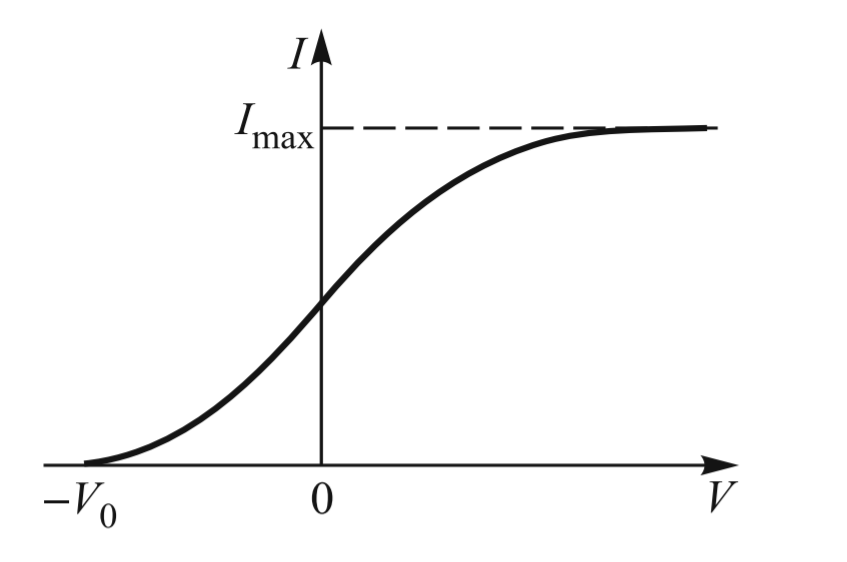
\includegraphics[width=11cm]{pics/I(V).png}
		\caption{Зависимость фототока от напряжения на аноде фотоэлемента}
		\label{VAC}
	\end{figure}

	
	Здесь $ E_{max} $ ---  максимальная кинетическая энергия электрона после выхода из фотокатода, $ W $ --- работа выхода электрона из катода. Реально энергетический спектр вылетевших из фотокатода электронов непрерывен --- он простирается от нуля до $ E_{max} $. 
	
	Для измерения энергии вылетевших фотоэлектронов вблизи фотокатода
	обычно располагается второй электрод
	(анод), на который подается задерживающий ($ V < 0 $) или ускоряющий ($ V >
	0 $) потенциал. При достаточно больших
	ускоряющих напряжениях фототок достигает насыщения (рис. \ref{VAC}): все испущенные электроны попадают на анод.
	
	При задерживающих потенциалах на анод попадают лишь электроны,
	обладающие достаточно большой кинетической энергией, в то время
	как медленно движущиеся электроны заворачиваются полем и возвращаются на катод. При некотором значении $ V = -V_0 $ (потенциал запирания) даже наиболее быстрые фотоэлектроны не могут достичь
	анода.
	Максимальная кинетическая энергия $ E_{max} $ электронов связана с
	запирающим потенциалом $ V_0 $ очевидным соотношением $ E_{max} = eV_0 $. Тогда \eqref{energy_bal} примет вид, называемый уравнением Эйнштейна:
	
	\begin{equation}\label{Einsteain}
		eV_0 = \hbar\omega - W 
	\end{equation}
	
	Чтобы определить величину запирающего
	напряжения, нам надо правильно экстраполировать получаемую токовую зависимость к нулю, т. е. определить, какова функциональная
	зависимость $ I(V) $. Расчет для простейшей геометрии --- плоский катод, освещаемый светом, и параллельный ему анод --- приводит к зависимости
	
	\begin{equation}\label{sqrt I = V}
		\sqrt{I} \propto V_0 - V
	\end{equation}
	
	т. е. корень квадратный из фототока линейно
	зависит от запирающего напряжения. Эта зависимость хорошо описывает экспериментальные данные.
	
	В работе изучается зависимость фототока из фотоэлемента от величины задерживающего потенциала $ V $ для различных частот света $ \omega $, лежащих в видимой области спектра. С целью экспериментальной
	проверки уравнения Эйнштейна определяются потенциалы запирания
	$ V_0 $ при разных частотах света и строится зависимость $ V_0(\omega) $, которая, как это следует из \eqref{Einsteain}, должна иметь вид
	
	\begin{equation}\label{V(w)}
		V_0 (\omega) = \dfrac{\hbar\omega - W}{e}
	\end{equation}
	
	\begin{figure}[h!]
		\centering
		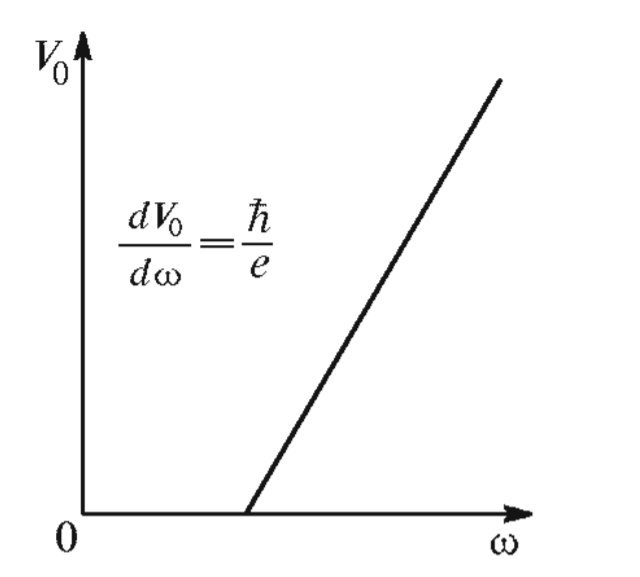
\includegraphics[width=11cm]{pics/V(w).png}
		\caption{Зависимость запирающего потенциала от частоты света}
		\label{dvdw}
	\end{figure}
	
	Потенциал запирания $ V_0 $ для любого катода линейно зависит от
	частоты света $ \omega $. По наклону прямой на графике $ V_0(\omega) $ (рис. \ref{dvdw}) можно определить постоянную Планка:
	
	\begin{equation}\label{dV/dw}
		\dfrac{dV_0}{d\omega} = \dfrac{\hbar}{e}
	\end{equation}
	
	Как показывает формула \eqref{dV/dw}, угол наклона прямой $ V_0(\omega) $ не зависит от рода вещества, из которого изготовлен фотокатод. От рода вещества, однако, зависит величина фототока, работа выхода $ W $ и форма кривой $ I(V) $ (рис. \ref{VAC}). Все это определяет выбор пригодных для
	опыта катодов.

	\section{Экспермиментальная установка}

	\begin{figure}[h!]
		\centering
		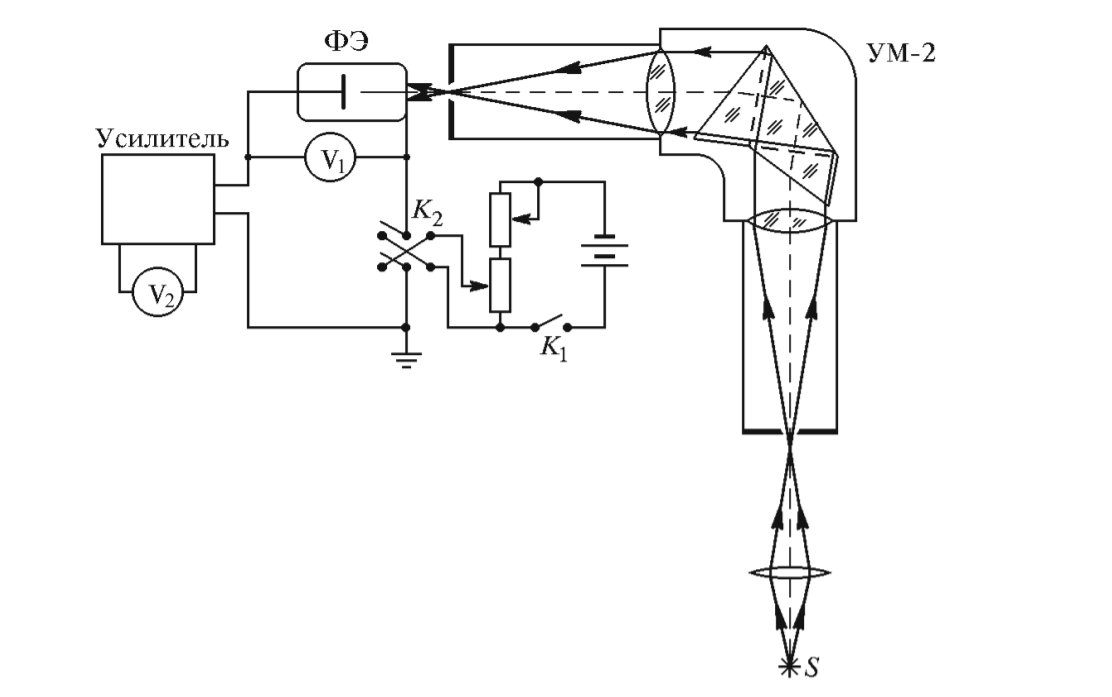
\includegraphics[width=11cm]{pics/scheme.png}
		\caption{Принципиальная схема экспериментальной установки}
		\label{scheme}
	\end{figure}

	Схема установки приведена на рисунке \ref{scheme}. Свет от источника $S$ с помощью конденсора фокусируется на входную щель
	призменного монохроматора УМ-2, выделяющего узкий спектральный интервал, и попадает на катод фотоэлемента ФЭ. 

	Фотоэлемент конструктивно представляет собой откачанный до высокого вакуума стеклянный баллон диаметром $25$ мм и высотой $30$ мм. 
	Внути баллона расположены два электрода: фотокатод и анод. Фотокатод представляет собой тонкую пленку металла, легированного элементами
	$Na$, $K$, $Sb$ и $C$ и расположенного на массивной металлической пластине. Анод фотоэлемента выполнен в виде пояска тонкой плекнкм, осажденной на внутренней части боковой поверхности вверху баллона.
	Такое расположениефотокатода и анода обеспечивает наиболее полный сбор на аноде электронов, эмитированных фотокатодом. Фотокатод и анд имеют вплавленные в стекло колбы никелевые выводы для подключения к внешней схеме.
	Такой фотоэлемент обладает спектральной чувствительностью в области длин влн от 300 до 850 нм. Наибольшая чувствительность ФЭ лежит в области от 400 до 500 нм. 

	Фототок, протекающий  фотоэлементе, мал, особенно при потенциалах $V$, близких к $V_0$, и не может быть измерен непосредственно. Для его измерения используется усилитель постяонного тока. Для уменьшения погрешностей измреений,
	обусловленных наводками, усилитель фототока смонтирован в одной корпуске с ФЭ.
	
	\section{Ход работы и обработка данных}

	Сначала выполним градуировку монохроматора. Проведем серию измерений для линий спектра неона, снимая зависимость длины волны света от параметра $ \theta $ барабана монохроматора.
	Результаты занесем в таблицу и используем в будущем для измерений.
	\begin{table}[h!]
        \centering
        \begin{tabular}{| c | c | c | c | c |}
\hline
$U, mV$ & $T_{room}, K$ & $T, K$ & $T_{br}, K$ & $ \sigma_{T}, K$\\
\hline
$39920$ & $298$ & $973,66$ & $1000$ & $ 28 $\\
\hline
\end{tabular}

        \caption{: данные для градуировочной кривой}
    	\label{tb_1}
	\end{table}

	Теперь проведем 5 серий измерений зависимости фототока от напряжения для разных длин волн падающего света, изменяя на монохроматоре параметр $ \theta $ и переводя его в длину волны с помощью градуировки.
	Результаты измерений сведем в таблицы.

	\begin{equation}\label{ols}
		a = \dfrac{\langle xy \rangle - \langle x \rangle \langle y \rangle}{\langle x^2 \rangle - \langle x \rangle^2}
	\end{equation}

	\begin{equation}\label{ols_err}
		\sigma_a = \dfrac{1}{\sqrt{n}}\sqrt{\dfrac{\langle y^2 \rangle - \langle y \rangle^2}{\langle x^2 \rangle - \langle x \rangle^2} - A^2}
	\end{equation}

	Зная наклона $\frac{dV_0}{d\omega}$ прямой и рассчитан погрешность МНК, найдем значение постоянной Дирака $\Rightarrow$ постоянной Планка:

	\[ \hbar = (\frac{dV_0}{d\omega} \pm \sigma_{\frac{dV_0}{d\omega}} ) \cdot e  \approx (0,46 \pm 0,056) \cdot 10^{-34} \text{Дж $\cdot$ c} \]

	\section{Вывод}

	Таким образом, в ходе выполнения работы мы убедились в явлении фотоэффекта и с помощью уравнения Эйнштейна измерили постоянную Дирака. 

	К сожалению измеренное значение постоянной Дирака отличается от табличного значения в пределах погрешности МНК приблизительно в два раза. Причин, объяснящих это, я нашел несколько: 
	
	\begin{itemize}
		\item неточное определение длин волны спектра неона
		\item недостаточно верная оценка погрешности измеряемых напряжений
	\end{itemize}
	
	
	\newpage

	\begin{table}[h!]
        \centering
        \begin{tabular}{| c | c | c | c | c |}
\hline
$\theta,^{\circ}$ & $U(I)$ & $V_{ФЭ}$ & $\sigma_{U(I)}$ & $\sigma_{V_{ФЭ}}$\\
\hline
$2404$ & $0,036$ & $0,302$ & $0,0004$ & $0,003$\\
\hline
$$ & $0,032$ & $0,262$ & $0,0004$ & $0,003$\\
\hline
$$ & $0,027$ & $0,202$ & $0,0004$ & $0,003$\\
\hline
$$ & $0,02$ & $0,121$ & $0,0004$ & $0,003$\\
\hline
$$ & $0,016$ & $0,039$ & $0,0004$ & $0,003$\\
\hline
$$ & $0,009$ & $-0,062$ & $0,0004$ & $0,003$\\
\hline
$$ & $0,006$ & $-0,162$ & $0,0004$ & $0,003$\\
\hline
$$ & $0$ & $-0,303$ & $0,0004$ & $0,003$\\
\hline
\end{tabular}

        \caption{: данные для ВАХ при $\lambda = 6402$ A}
    	\label{tb_2}
	\end{table}

	\begin{figure}[h!]
		\centering
		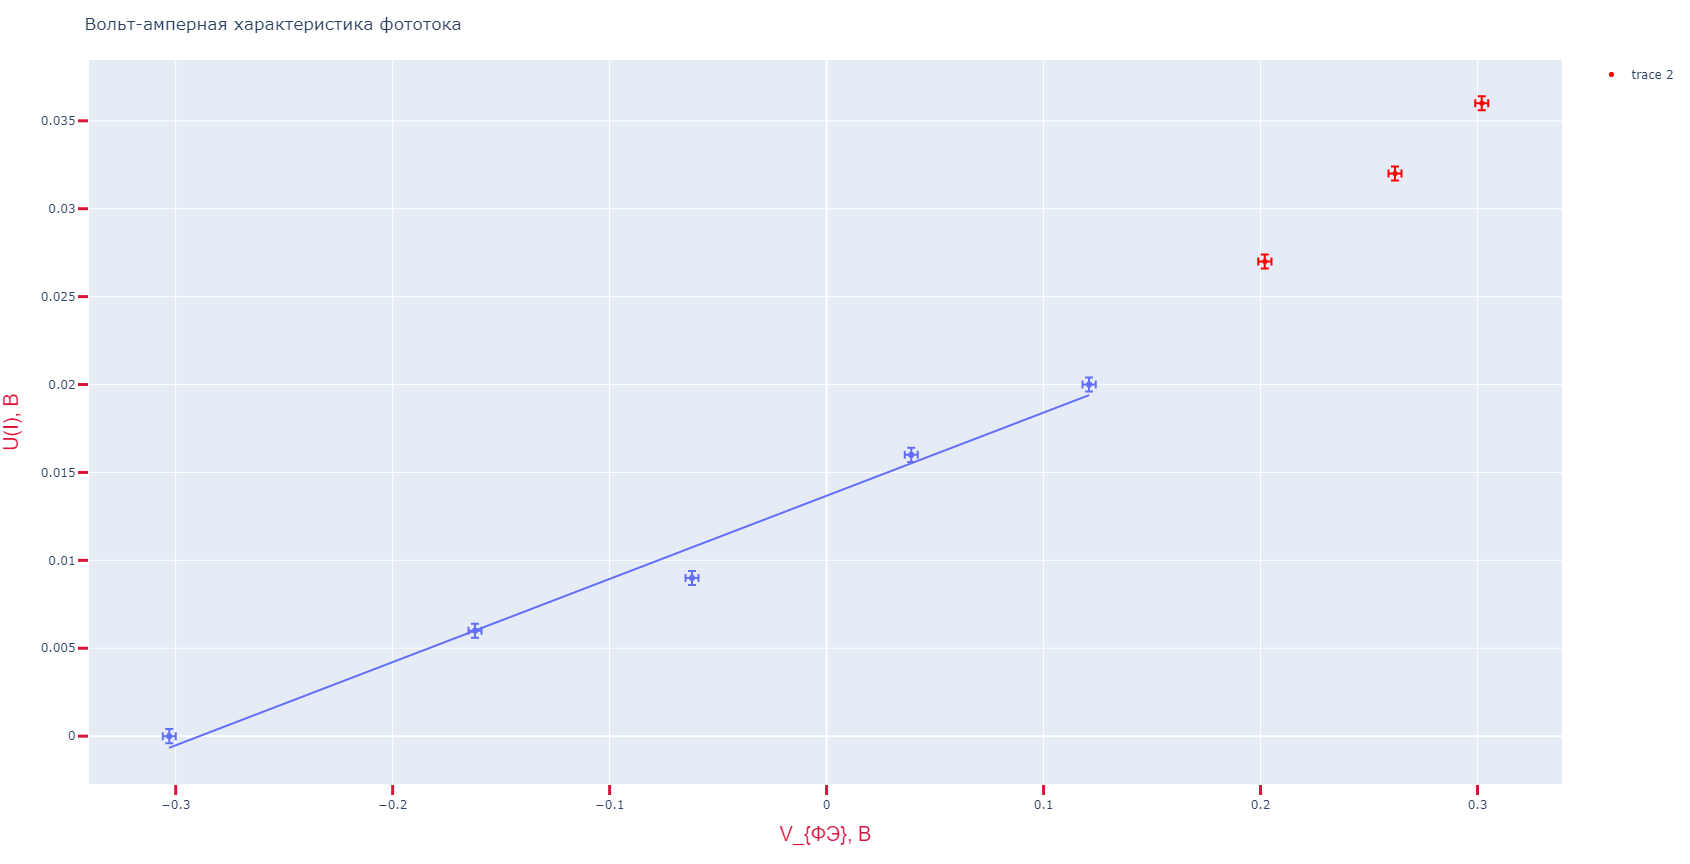
\includegraphics[width=1.0\linewidth]{pics/vac_1.png}
		\caption{Вольт-амперная характеристика  для таблицы \ref{tb_2}}
		\label{vac1}
	\end{figure}

	\newpage

	\begin{table}[h!]
        \centering
        \begin{tabular}{| c | c |}
\hline
$ln(T_{term})$ & $ln(P)$\\
\hline
$6,82$ & $2,43$\\
\hline
$6,96$ & $2,88$\\
\hline
$7,05$ & $3,42$\\
\hline
$7,15$ & $3,73$\\
\hline
$7,22$ & $3,98$\\
\hline
$7,31$ & $4,25$\\
\hline
$7,38$ & $4,48$\\
\hline
$7,4$ & $4,72$\\
\hline
$7,48$ & $4,88$\\
\hline
$7,51$ & $5,1$\\
\hline
$7,55$ & $5,29$\\
\hline
\end{tabular}

        \caption{: данные для ВАХ при $\lambda = 6096$ A}
    	\label{tb_3}
	\end{table}

	\begin{figure}[h!]
		\centering
		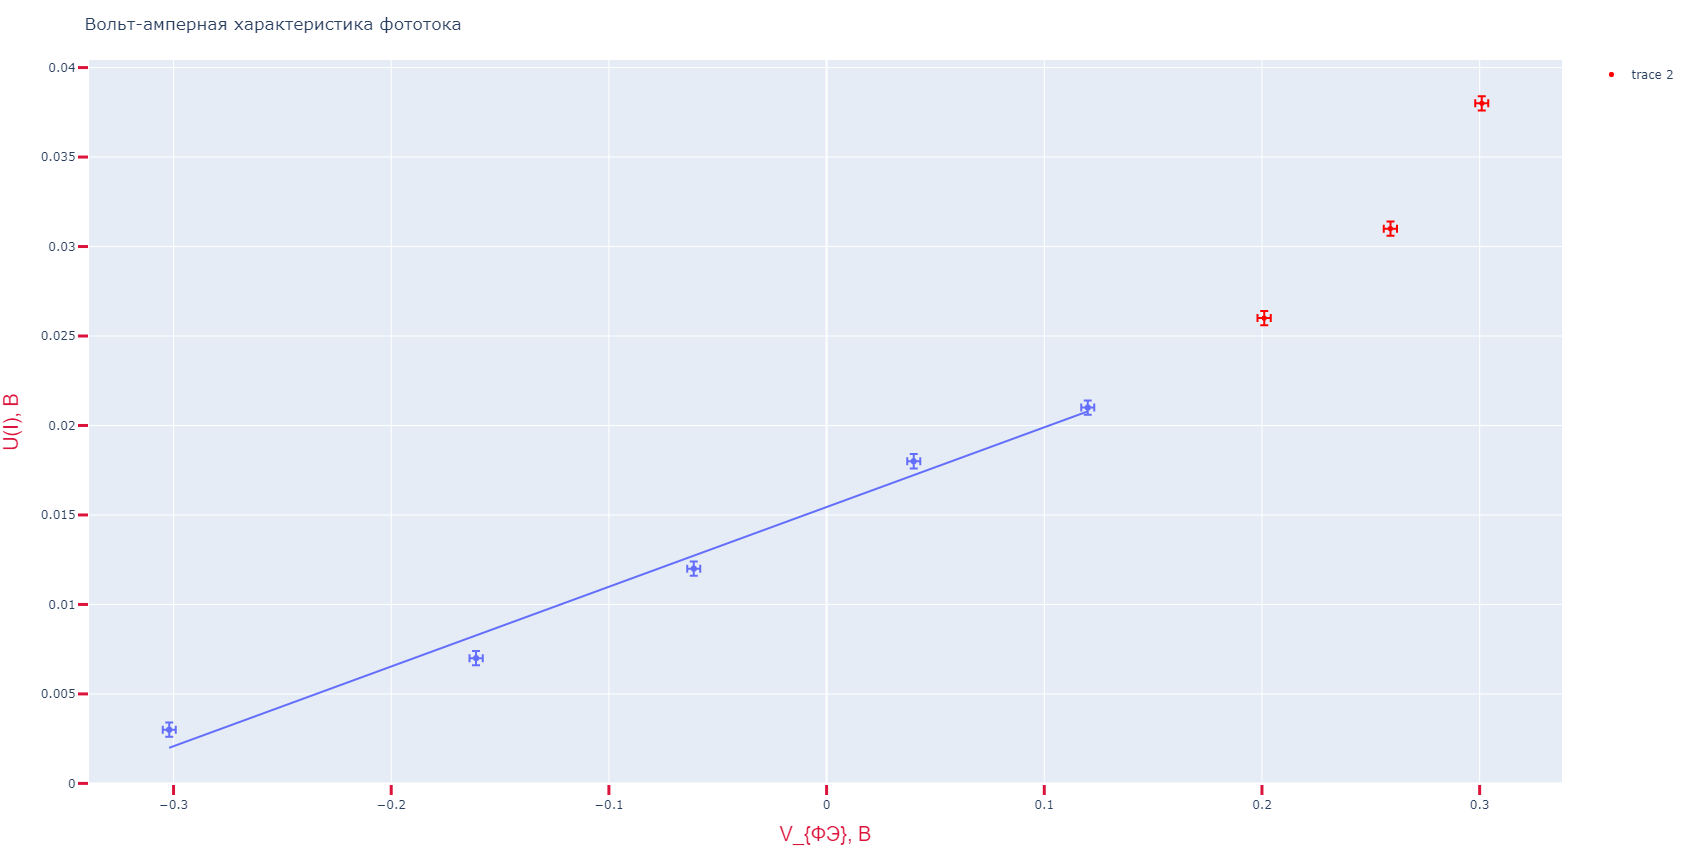
\includegraphics[width=1.0\linewidth]{pics/vac_2.png}
		\caption{Вольт-амперная характеристика для таблицы \ref{tb_3}}
		\label{vac2}
	\end{figure}

	\newpage


	\begin{table}[h!]
        \centering
        \begin{tabular}{| c | c | c | c |}
\hline
$d, cm$ & $ln(N_0/N)$ & $\sigma_{d}, см$ & $\sigma_{ln(N_0/N)}$\\
\hline
$2$ & $0,54$ & $0,01$ & $0,042$\\
\hline
$3,99$ & $1,05$ & $0,01$ & $0,042$\\
\hline
$5,99$ & $1,54$ & $0,01$ & $0,042$\\
\hline
$8$ & $2,02$ & $0,01$ & $0,042$\\
\hline
$10,01$ & $2,44$ & $0,01$ & $0,042$\\
\hline
$12$ & $2,89$ & $0,01$ & $0,042$\\
\hline
\end{tabular}

        \caption{: данные для ВАХ при $\lambda = 5852$ A}
    	\label{tb_4}
	\end{table}

	\begin{figure}[h!]
		\centering
		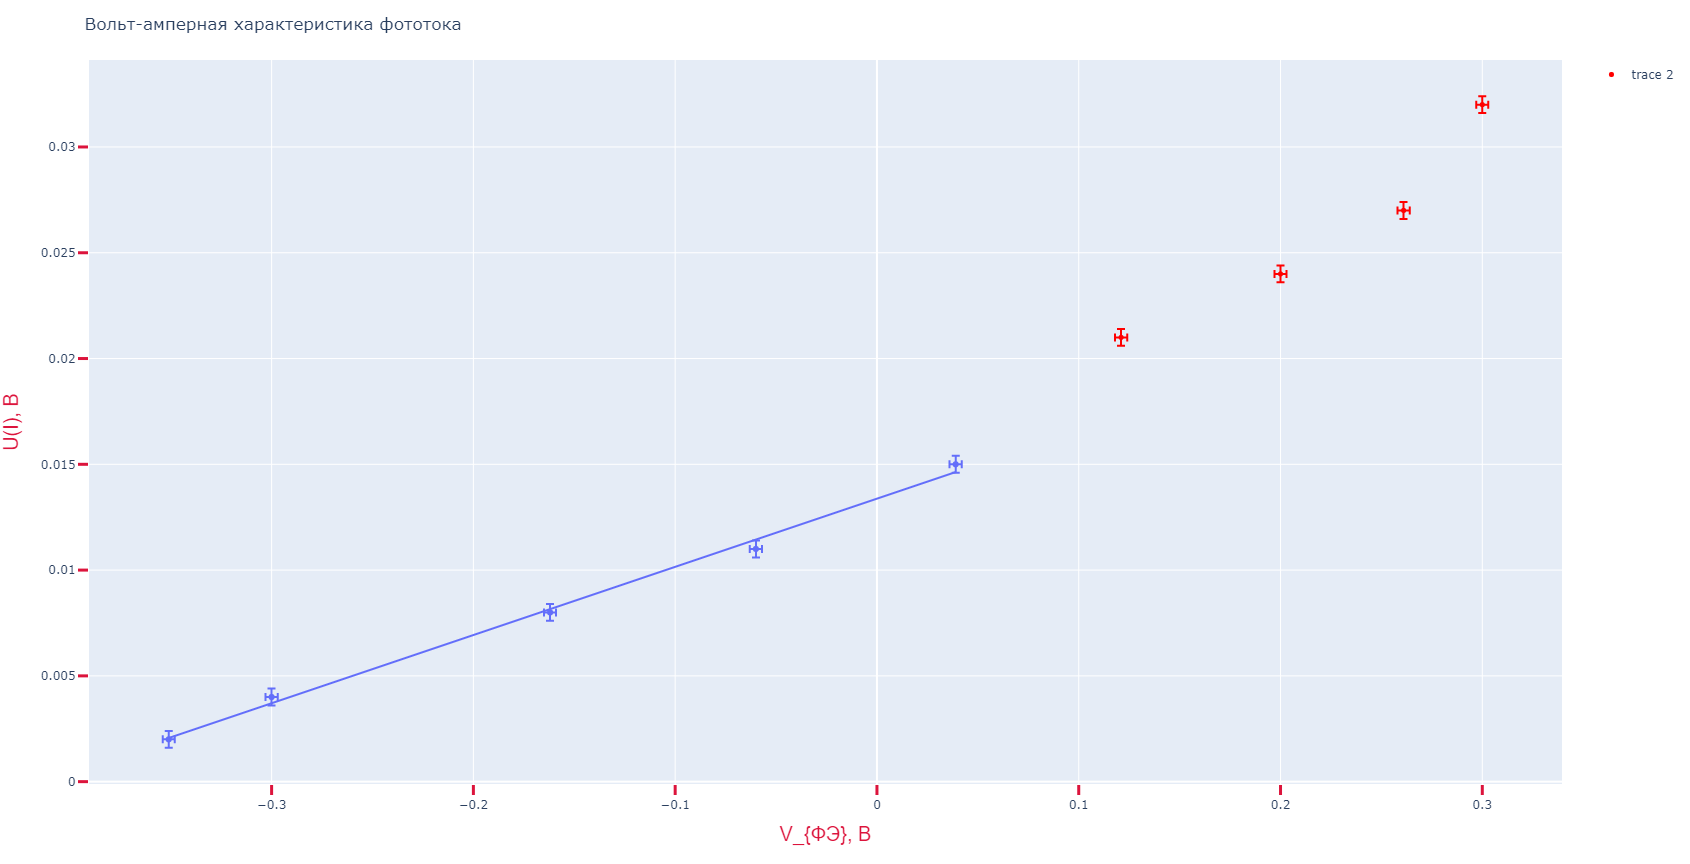
\includegraphics[width=1.0\linewidth]{pics/vac_3.png}
		\caption{Вольт-амперная характеристика  для таблицы \ref{tb_4}}
		\label{vac3}
	\end{figure}

	\newpage


	\begin{table}[h!]
        \centering
        \begin{tabular}{| c | c | c | c | c |}
\hline
$\theta,^{\circ}$ & $U(I)$ & $V_{ФЭ}$ & $\sigma_{U(I)}$ & $\sigma_{V_{ФЭ}}$\\
\hline
$2500$ & $0,514$ & $7$ & $0,005$ & $0,07$\\
\hline
$$ & $0,5$ & $5,999$ & $0,005$ & $0,07$\\
\hline
$$ & $0,48$ & $5$ & $0,005$ & $0,07$\\
\hline
$$ & $0,472$ & $4,495$ & $0,005$ & $0,07$\\
\hline
$$ & $0,456$ & $3,999$ & $0,005$ & $0,07$\\
\hline
$$ & $0,434$ & $3,505$ & $0,005$ & $0,07$\\
\hline
$$ & $0,406$ & $2,998$ & $0,005$ & $0,07$\\
\hline
$$ & $0,36$ & $2,5$ & $0,005$ & $0,07$\\
\hline
$$ & $0,273$ & $1,998$ & $0,005$ & $0,07$\\
\hline
$$ & $0,165$ & $1,49$ & $0,005$ & $0,07$\\
\hline
$$ & $0,13$ & $1,25$ & $0,005$ & $0,07$\\
\hline
$$ & $0,087$ & $1,002$ & $0,005$ & $0,07$\\
\hline
$$ & $0,06$ & $0,75$ & $0,005$ & $0,07$\\
\hline
$$ & $0,038$ & $0,5$ & $0,005$ & $0,07$\\
\hline
$$ & $0,021$ & $0,249$ & $0,005$ & $0,07$\\
\hline
$$ & $0,013$ & $0,1$ & $0,005$ & $0,07$\\
\hline
$$ & $0,008$ & $0,009$ & $0,005$ & $0,07$\\
\hline
$$ & $0,006$ & $-0,05$ & $0,005$ & $0,07$\\
\hline
$$ & $0,003$ & $-0,1$ & $0,005$ & $0,07$\\
\hline
$$ & $0,002$ & $-0,15$ & $0,005$ & $0,07$\\
\hline
$$ & $0,001$ & $-0,2$ & $0,005$ & $0,07$\\
\hline
$$ & $0$ & $-0,249$ & $0,005$ & $0,07$\\
\hline
\end{tabular}

        \caption{: данные для ВАХ при $\lambda = 6678$ A}
    	\label{tb_5}
	\end{table}

	\begin{figure}[h!]
		\centering
		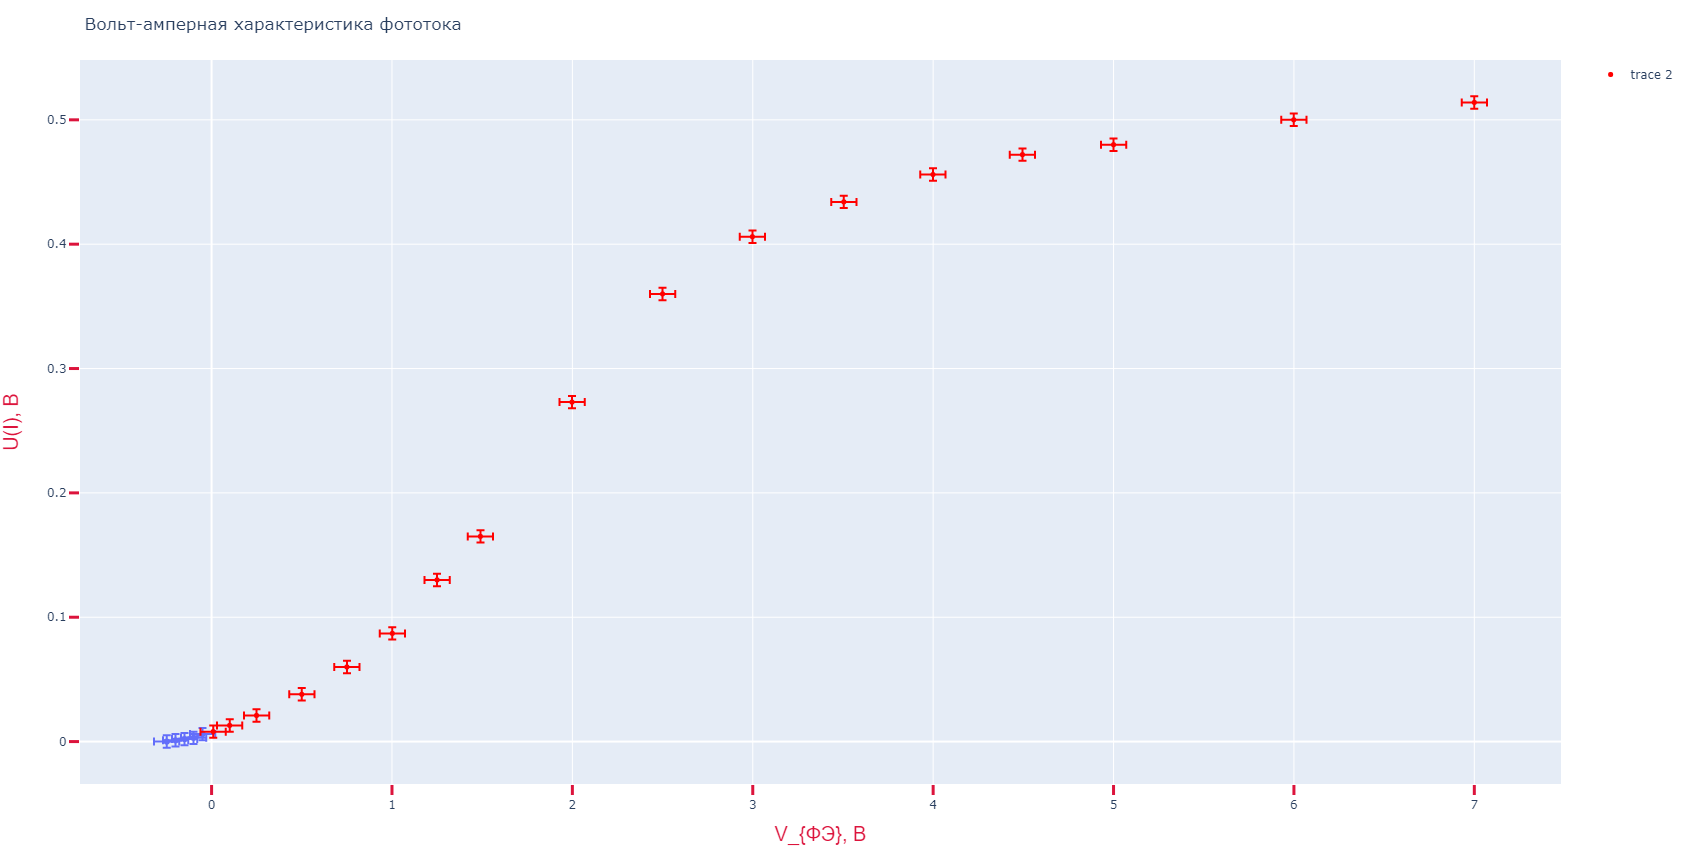
\includegraphics[width=1.0\linewidth]{pics/vac_4.png}
		\caption{Вольт-амперная характеристика  для таблицы \ref{tb_5}}
		\label{vac4}
	\end{figure}

	\newpage


	\begin{table}[h!]
        \centering
        \begin{tabular}{| c | c | c | c | c |}
\hline
$\theta, ^{\circ}$ & $U(I)$ & $V_{ФЭ}$ & $\sigma_{U(I)}$ & $\sigma_{V_{ФЭ}}$\\
\hline
$2162$ & $0,49$ & $7,46$ & $0,005$ & $0,07$\\
\hline
$$ & $0,487$ & $7,377$ & $0,005$ & $0,07$\\
\hline
$$ & $0,481$ & $7,003$ & $0,005$ & $0,07$\\
\hline
$$ & $0,47$ & $6,504$ & $0,005$ & $0,07$\\
\hline
$$ & $0,462$ & $6$ & $0,005$ & $0,07$\\
\hline
$$ & $0,45$ & $5,508$ & $0,005$ & $0,07$\\
\hline
$$ & $0,43$ & $5,005$ & $0,005$ & $0,07$\\
\hline
$$ & $0,41$ & $4,5$ & $0,005$ & $0,07$\\
\hline
$$ & $0,383$ & $4,003$ & $0,005$ & $0,07$\\
\hline
$$ & $0,343$ & $3,5$ & $0,005$ & $0,07$\\
\hline
$$ & $0,281$ & $3$ & $0,005$ & $0,07$\\
\hline
$$ & $0,215$ & $2,503$ & $0,005$ & $0,07$\\
\hline
$$ & $0,156$ & $2,001$ & $0,005$ & $0,07$\\
\hline
$$ & $0,127$ & $1,75$ & $0,005$ & $0,07$\\
\hline
$$ & $0,103$ & $1,5$ & $0,005$ & $0,07$\\
\hline
$$ & $0,084$ & $1,25$ & $0,005$ & $0,07$\\
\hline
$$ & $0,075$ & $1,125$ & $0,005$ & $0,07$\\
\hline
$$ & $0,066$ & $1$ & $0,005$ & $0,07$\\
\hline
$$ & $0,059$ & $0,9$ & $0,005$ & $0,07$\\
\hline
$$ & $0,051$ & $0,8$ & $0,005$ & $0,07$\\
\hline
$$ & $0,045$ & $0,7$ & $0,005$ & $0,07$\\
\hline
$$ & $0,033$ & $0,6$ & $0,005$ & $0,07$\\
\hline
$$ & $0,031$ & $0,5$ & $0,005$ & $0,07$\\
\hline
$$ & $0,027$ & $0,4$ & $0,005$ & $0,07$\\
\hline
$$ & $0,017$ & $0,2$ & $0,005$ & $0,07$\\
\hline
$$ & $0,013$ & $0,1$ & $0,005$ & $0,07$\\
\hline
$$ & $0,009$ & $0,01$ & $0,005$ & $0,07$\\
\hline
$$ & $0,005$ & $-0,1$ & $0,005$ & $0,07$\\
\hline
$$ & $0,002$ & $-0,2$ & $0,005$ & $0,07$\\
\hline
$$ & $0$ & $-0,3$ & $0,005$ & $0,07$\\
\hline
\end{tabular}

        \caption{: данные для ВАХ при $\lambda = 6507$ A}
    	\label{tb_6}
	\end{table}

	\begin{figure}[h!]
		\centering
		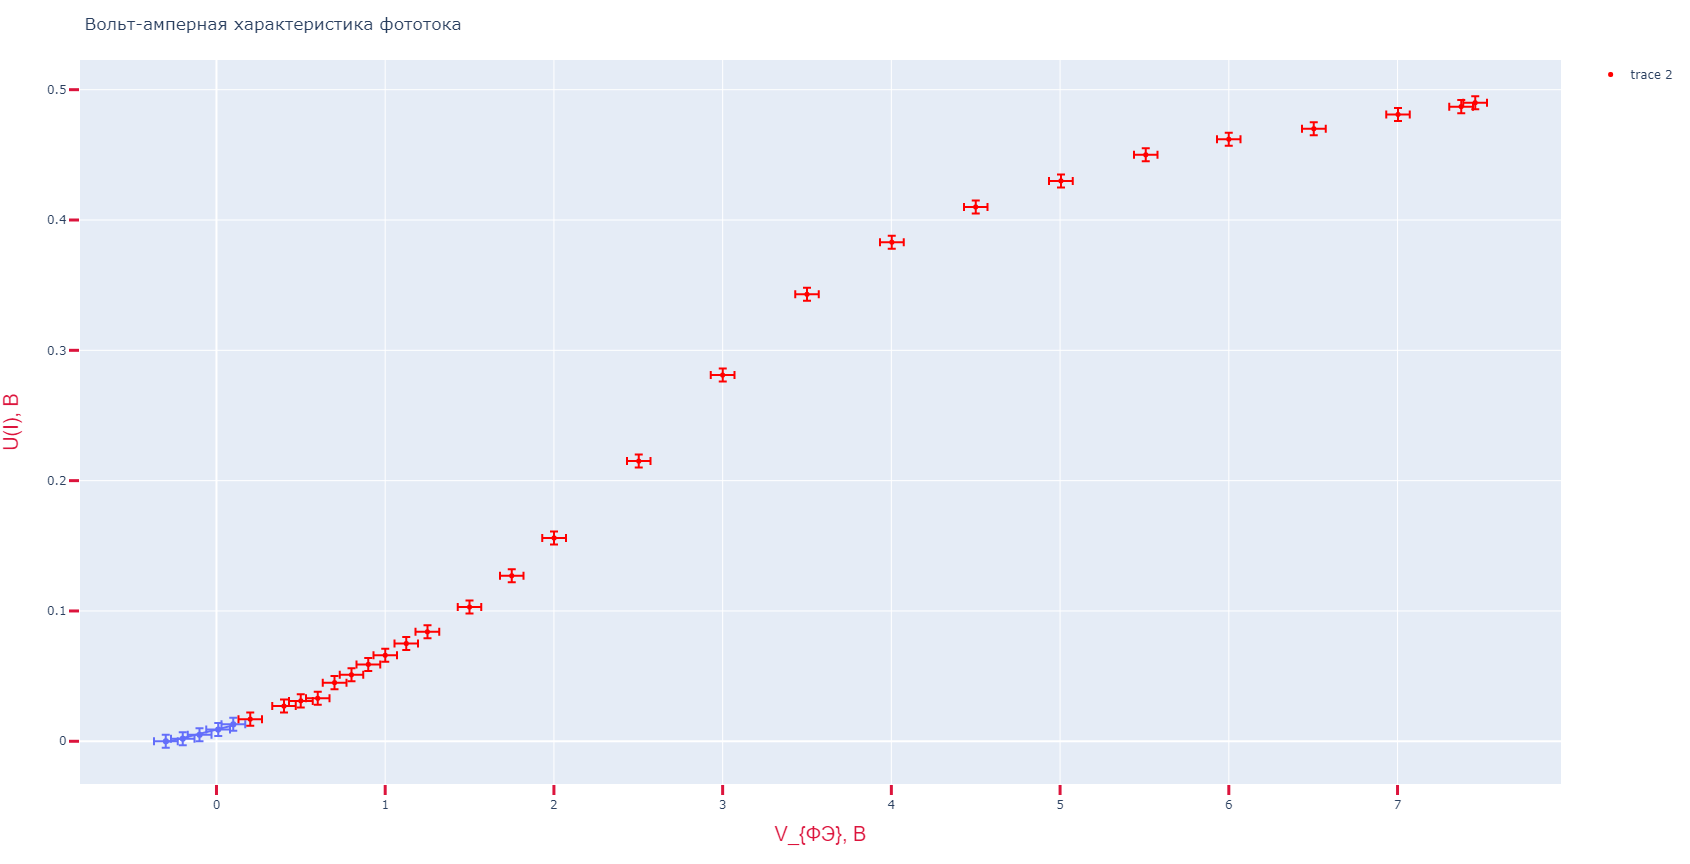
\includegraphics[width=1.0\linewidth]{pics/vac_5.png}
		\caption{Вольт-амперная характеристика для таблицы \ref{tb_6}}
		\label{vac5}
	\end{figure}

	\newpage


	\begin{table}[h!]
        \centering
        \begin{tabular}{| c | c | c |}
\hline
$образец$ & $\mu , 1/c$ & $\sigma_{\mu}, 1/c$\\
\hline
$Al$ & $0,234$ & $0,0038$\\
\hline
$Pb$ & $1,29$ & $0,0536$\\
\hline
$Fe$ & $0,641$ & $0,0618$\\
\hline
\end{tabular}

        \caption{: данные построения зависимости запирающего потенциала от часоты света}
    	\label{tb_7}
	\end{table}

	\begin{figure}[h!]
		\centering
		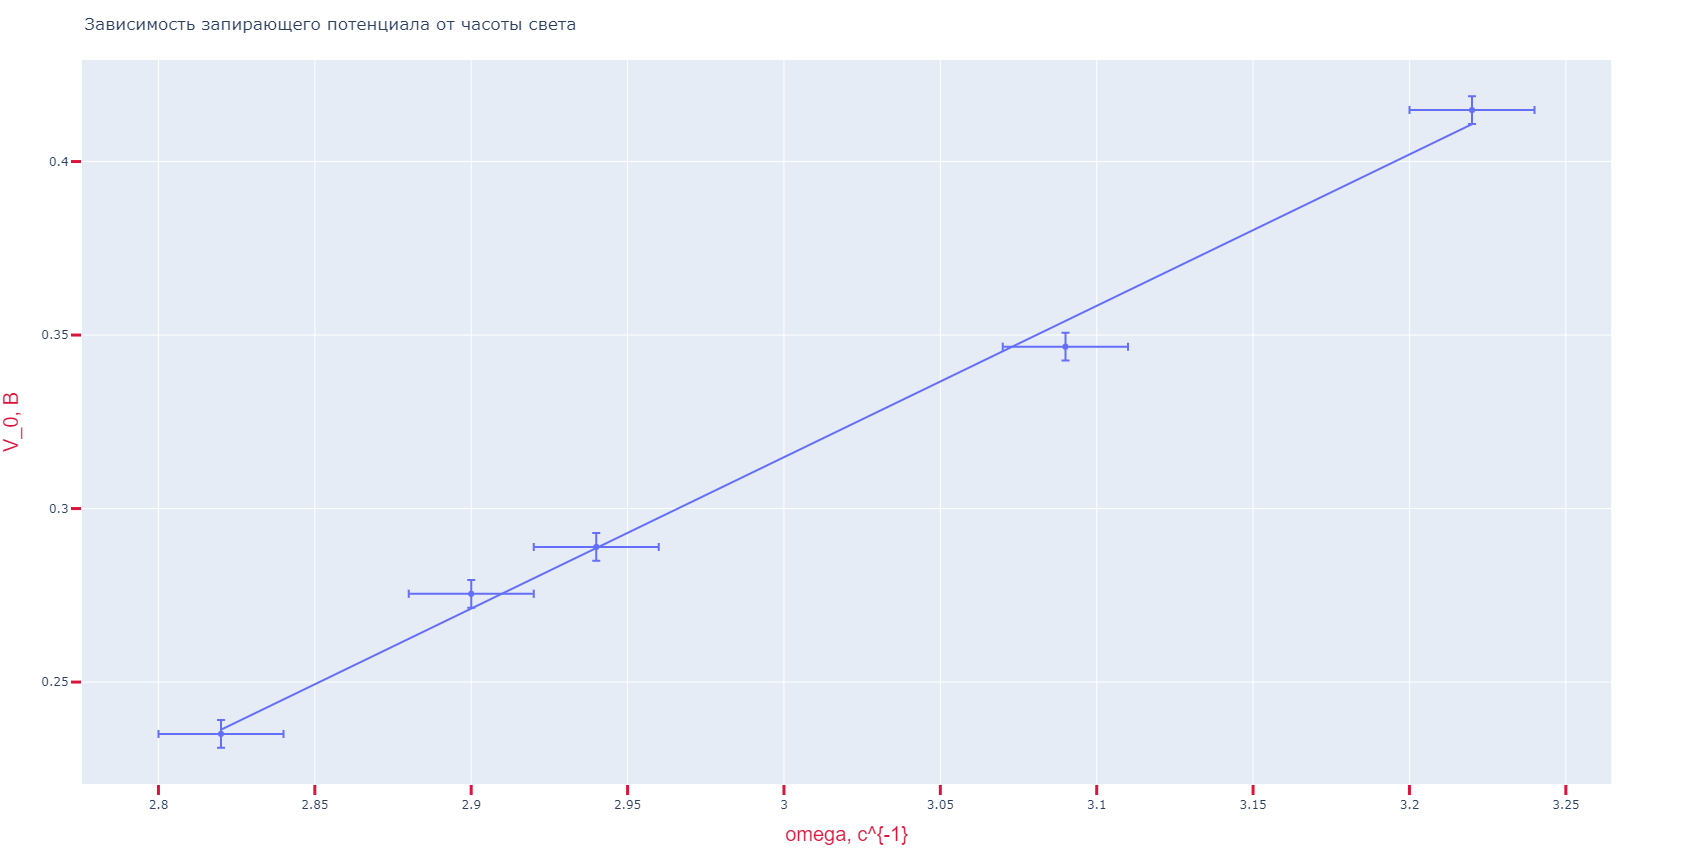
\includegraphics[width=1.0\linewidth]{pics/h_calc.png}
		\caption{Вольтамперная характеристика}
		\label{h_calc}
	\end{figure}


\end{document}
